% Options for packages loaded elsewhere
\PassOptionsToPackage{unicode}{hyperref}
\PassOptionsToPackage{hyphens}{url}
%
\documentclass[
]{article}
\usepackage{amsmath,amssymb}
\usepackage{iftex}
\ifPDFTeX
  \usepackage[T1]{fontenc}
  \usepackage[utf8]{inputenc}
  \usepackage{textcomp} % provide euro and other symbols
	\usepackage{fontspec}

	\else % if luatex or xetex
  \usepackage{unicode-math} % this also loads fontspec
	\usepackage{fontspec}
	\usepackage{newunicodechar}
	\newfontface{\freesans}{FreeSans}
	\newunicodechar{◈}{{\freesans{◈}}}
  \defaultfontfeatures{Scale=MatchLowercase}
  \defaultfontfeatures[\rmfamily]{Ligatures=TeX,Scale=1}
\fi
\usepackage{lmodern}
\ifPDFTeX\else
  % xetex/luatex font selection
\fi
% Use upquote if available, for straight quotes in verbatim environments
\IfFileExists{upquote.sty}{\usepackage{upquote}}{}
\IfFileExists{microtype.sty}{% use microtype if available
  \usepackage[]{microtype}
  \UseMicrotypeSet[protrusion]{basicmath} % disable protrusion for tt fonts
}{}
\makeatletter
\@ifundefined{KOMAClassName}{% if non-KOMA class
  \IfFileExists{parskip.sty}{%
    \usepackage{parskip}
  }{% else
    \setlength{\parindent}{0pt}
    \setlength{\parskip}{6pt plus 2pt minus 1pt}}
}{% if KOMA class
  \KOMAoptions{parskip=half}}
\makeatother
\usepackage{xcolor}
\usepackage[margin=1in]{geometry}
\usepackage{graphicx}
\makeatletter
\def\maxwidth{\ifdim\Gin@nat@width>\linewidth\linewidth\else\Gin@nat@width\fi}
\def\maxheight{\ifdim\Gin@nat@height>\textheight\textheight\else\Gin@nat@height\fi}
\makeatother
% Scale images if necessary, so that they will not overflow the page
% margins by default, and it is still possible to overwrite the defaults
% using explicit options in \includegraphics[width, height, ...]{}
\setkeys{Gin}{width=\maxwidth,height=\maxheight,keepaspectratio}
% Set default figure placement to htbp
\makeatletter
\def\fps@figure{htbp}
\makeatother
\setlength{\emergencystretch}{3em} % prevent overfull lines
\providecommand{\tightlist}{%
  \setlength{\itemsep}{0pt}\setlength{\parskip}{0pt}}
\setcounter{secnumdepth}{-\maxdimen} % remove section numbering
\let\oldsection\section
\renewcommand{\section}[1]{\clearpage\oldsection{#1}}
  \def\tightlist{}
\ifLuaTeX
  \usepackage{selnolig}  % disable illegal ligatures
\fi
\usepackage{bookmark}
\IfFileExists{xurl.sty}{\usepackage{xurl}}{} % add URL line breaks if available
\urlstyle{same}
\hypersetup{
  hidelinks,
  pdfcreator={LaTeX via pandoc}}

\author{}
\date{}

\begin{document}

\section{Complex Numbers}\label{complex-numbers}

\subsection{Super brief history of
numbers}\label{super-brief-history-of-numbers}

Leopold Kronecker, 19th century German mathematician, is credited with
saying (in German)\footnote{``Die ganzen Zahlen hat der liebe Gott
  gemacht, alles andere ist Menschenwerk''} ``Whole numbers were made by
God, all else is the work of man.'' If you think about it, whole numbers
are great for counting but, one day, somebody had to solve an equation
like \(2x=1\) and this required the invention of (discovery of?)
rational numbers. These were great for a while until someone had to
solve \(x^2 = 2\).\footnote{We believe they were finding the diagonal of
  a unit square}. So a new number, ◈, was born (they didn't really use
the symbol ◈ but we have to call it something.) So ◈squared equals 2. The first
algebraic number, \(\sqrt2\) was soon found to be like \(\sqrt3\) and
\(\sqrt[3]5\) and it was discovered how to add and multiply these things
together. And everyone was happy. Until some wise guy tried to solve
\(x^2 = -1\). And then there was trouble.

\subsection{Complex Numbers}\label{complex-numbers-1}

Just like a symbol (in our questionable history above) was created to
indicate \(\sqrt2\), a symbol was introduced to mean \(\sqrt{-1}\). That
symbol is, of course \(i\). \(i\) is the imaginary unit. Multiples of
\(i\) are imaginary numbers. And when imaginary and real numbers are
added togther, a complex number is born. A complex number is a number
that can be expressed in the form \(a + bi\), where \(a\) and \(b\) are
real numbers, and \(i\) is the imaginary unit with the property that
\(i^2 = -1\). The real part of the complex number is \(a\), and the
imaginary part is \(b\). Complex numbers extend the concept of
one-dimensional number lines to a two-dimensional complex plane, and a
whole new world of mathematical possibilities arises.

\textbf{Example} The complex number \(3 + 4i\) has a real part of 3 and
an imaginary part of 4.

\begin{figure}
\centering
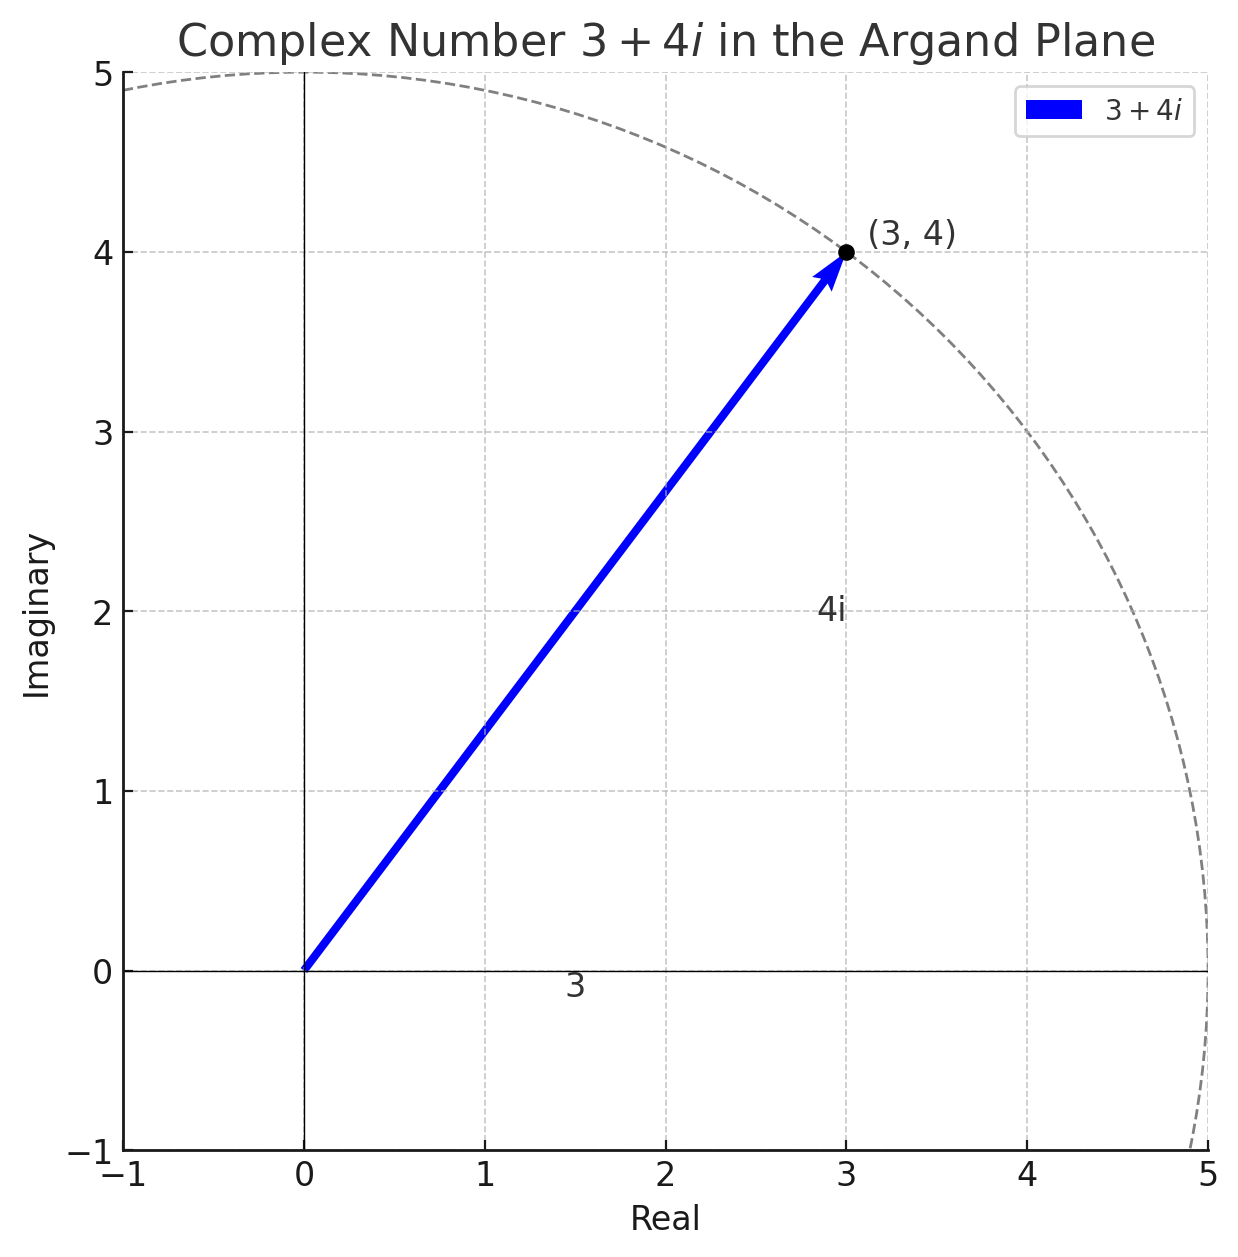
\includegraphics[width=0.33\textwidth,height=\textheight]{complex-number.png}
\caption{A complex number}
\end{figure}

In the complex plane, also known as the Argand plane, complex numbers
are represented as points or vectors. The horizontal axis represents the
real part, and the vertical axis represents the imaginary part.

\textbf{Example} The complex number \(3 + 4i\) is represented as a point
(3, 4) in the complex plane, or as a vector from the origin (0, 0) to
the point (3, 4).

\subsection{Basic Operations}\label{basic-operations}

\subsubsection{Addition and Subtraction}\label{addition-and-subtraction}

Adding or subtracting complex numbers involves combining their real
parts and their imaginary parts separately.

\textbf{Example - Addition} Given \(z_1 = 3 + 4i\) and \(z_2 = 1 + 2i\),
\(z_1 + z_2 = (3 + 1) + (4i + 2i) = 4 + 6i\).

\textbf{Example - Subtraction} Given \(z_1 = 3 + 4i\) and
\(z_2 = 1 + 2i\), \(z_1 - z_2 = (3 - 1) + (4i - 2i) = 2 + 2i\).

\subsubsection{Magnitude (Modulus)}\label{magnitude-modulus}

The magnitude (or modulus) of a complex number is the distance from the
origin to the point in the complex plane, calculated as
\(\sqrt{a^2 + b^2}\).

\textbf{Example} For \(z = 3 + 4i\), Magnitude
\(|z| = \sqrt{3^2 + 4^2} = \sqrt{9 + 16} = \sqrt{25} = 5\).

\subsubsection{Direction (Argument)}\label{direction-argument}

The direction (or argument) of a complex number is the angle formed with
the positive real axis. It can be found using the arctan function. Be
aware that this is the same process as converting rectangular
coordinates to polar coordinates. You will need to be aware of the
correct quadrant for your angle.

\textbf{Example} Find the argument of the complex number
\(12 + 4\sqrt{3}i\). \textbf{Solution} Argument
\(\theta = \tan^{-1}\left(\frac{4\sqrt{3}}{12}\right) = \tan^{-1}\left(\frac{\sqrt{3}}{3}\right) = \dfrac{\pi}{6}\).

\textbf{Example} Find the argument of the complex number
\(-\sqrt{2}+\sqrt{6}i\). \textbf{Solution} Argument
\(\theta = \tan^{-1}\left(\frac{\sqrt6}{-\sqrt2}\right) = \tan^{-1}\left(-\sqrt3\right) = -\tan^{-1}\left(\sqrt3\right) = \dfrac{-\pi}{3}\).
But the original point is in Quadrant II and this angle is Quadrant IV.
To fix, we add \(\pi\) radians:
\(\theta = \pi + \dfrac{-\pi}{3} = \dfrac{2\pi}{3}\).

\subsubsection{Multiplication}\label{multiplication}

Multiplication can be performed by treating complex number as binomials
and using the fact that \(i^2 = -1\). Here's a detailed example.
Consider two complex numbers: - \(z_1 = 1 + 2i\) - \(z_2 = 3 + 4i\)

To multiply these complex numbers, we multiply the binomials using the
distributive property:

\[
z_1 \cdot z_2 = (1 + 2i)(3 + 4i) = 1\cdot3 + 1\cdot4i + 2i\cdot3 + 2i\cdot4i = 3 + 4i + 6i + 8i^2
\]

We can combine like terms and use \(i^2 = -1\) to simplify:

\[
3 + 4i + 6i - 8 = -5 + 10i
\]

So, the product \(z_1 \cdot z_2 = -5 + 10i\).

\subsubsection{Division}\label{division}

To divide one complex number by another, you essentially perform
multiplication by the reciprocal of the divisor, just as with real
numbers. The key to simplifying such division is to eliminate the
imaginary part from the denominator, which is achieved by multiplying
both the numerator and the denominator by the conjugate of the
denominator.

The \textbf{conjugate} of a complex number \(a + bi\) is \(a - bi\).
Multiplying a complex number by its conjugate results in a real number,
specifically \(a^2 + b^2\), since
\((a + bi)(a - bi) = a^2 - (bi)^2 = a^2 + b^2\). This is the same term
you have seen applied to radicals: the conjugate of \(1+3\sqrt2\) is
\(1-3\sqrt2\) because the product of these two numbers is rational
\((1+3\sqrt2)(1-3\sqrt2) = 1-18 = -17\)

Given two complex numbers, \(z_1 = a + bi\) and \(z_2 = c + di\), to
find \(z_1 / z_2\), follow these steps:

\begin{enumerate}
\def\labelenumi{\arabic{enumi}.}
\tightlist
\item
  \textbf{Find the conjugate} of the denominator \(z_2\), which is
  \(c - di\).
\item
  \textbf{Multiply} both the numerator \(z_1\) and the denominator
  \(z_2\) by this conjugate.
\item
  \textbf{Simplify} the resulting expression to get the quotient in
  standard \(a + bi\) form.
\end{enumerate}

\textbf{Example} Divide \(z_1 = 1 + i\) by \(z_2 = 3 + 2i\).
\textbf{Solution:}

\begin{enumerate}
\def\labelenumi{\arabic{enumi}.}
\item
  \textbf{Conjugate of \(z_2\)}: The conjugate of \(3 + 2i\) is
  \(3 - 2i\).
\item
  \textbf{Multiply}: Multiply both \(z_1\) and \(z_2\) by \(3 - 2i\):

  \[
  \frac{1 + i}{3 + 2i} \times \frac{3 - 2i}{3 - 2i} = \frac{(1 + i)(3 - 2i)}{(3 + 2i)(3 - 2i)}
  \]
\item
  \textbf{Simplify}:

  \[
  \frac{3 - 2i + 3i - 2i^2}{9 - 6i + 6i - 4i^2} = \frac{3 + i - 2(-1)}{9 + 4} = \frac{5 + i}{13}
  \]

  Finally, divide each part by 13:

  \[
  \frac{5}{13} + \frac{1}{13}i
  \]
\end{enumerate}

\textbf{Example} Divide \(z_1 = 4 - i\) by \(z_2 = 1 - 2i\).
\textbf{Solution:}

\begin{enumerate}
\def\labelenumi{\arabic{enumi}.}
\item
  \textbf{Conjugate of \(z_2\)}: The conjugate is \(1 + 2i\).
\item
  \textbf{Multiply}:

  \[
  \frac{4 - i}{1 - 2i} \times \frac{1 + 2i}{1 + 2i} = \frac{(4 - i)(1 + 2i)}{(1 - 2i)(1 + 2i)}
  \]
\item
  \textbf{Simplify}:

  \[
  \frac{4 + 8i - i - 2i^2}{1 + 2i - 2i - 4i^2} = \frac{4 + 7i + 2}{1 + 4} = \frac{6 + 7i}{5}
  \]

  Simplifying further:

  \[
  \frac{6}{5} + \frac{7}{5}i
  \]
\end{enumerate}

\subsection{Polar Form of Complex
Numbers}\label{polar-form-of-complex-numbers}

First a quick review.

\textbf{Problem:} Convert the vectors \(\vec{a} = \langle -1,1 \rangle\)
and \(\vec{b} = \langle 6,-2\sqrt3 \rangle\) to polar form.

\textbf{Solution:} \(a =  \langle \sqrt2, \frac{3\pi}{4} \rangle\) and
\(b =  \langle 4\sqrt3, \frac{5\pi}{6} \rangle\)

In the complex plane, complex numbers can be represented as vectors, in
either rectangular or polar form. A complex number like \(z=-1 + i\) is
equivalent to the vector \(\langle -1, 1 \rangle\) in rectangular
coordinates. Since this vector has a magnitude of \(\sqrt{2}\) and an
argument of \(\dfrac{3\pi}{4}\), it can be represented in polar form
with \(r = \sqrt2\) and \(\theta=\dfrac{3\pi}{4}\). The
\textbf{notation} for this polar complex number is
\(z=\sqrt2 e^{i \cdot 3\pi/4}\). In the same way, the complex number
\(6-2\sqrt3 i = 4\sqrt3 e^{i \cdot 5\pi/6}\).

\paragraph{About polar form}\label{about-polar-form}

If a complex number \(z=a+bi\) has a magnitude of \(r\) and an argument
of \(\theta\), it can be written in polar form as \(z = r e^{i \theta}\)
where \(r^2 = a^2 + b^2\) and \(\tan \theta = \frac{b}{a}\). Why such a
strange formula? It is a consequence of the \emph{Euler Identity} which
defines complex exponentials (raising \(e\) to an imaginary power) as

\[e^{i\theta} = \cos \theta + i \sin \theta\]

For example, \(e^{i \pi/4} = \frac{\sqrt2}{2} + \frac{\sqrt2}{2}i\) and
\(4e^{2i \pi/3} = 4\left( \frac{-\sqrt3}{2} + \frac12 i \right ) = -2\sqrt{3} + 2 i\)

\paragraph{An example of
multiplication}\label{an-example-of-multiplication}

\paragraph{Finding the Argument of Each
Vector}\label{finding-the-argument-of-each-vector}

The argument of a complex number \(z = a + bi\) is given by
\(\theta = \tan^{-1}\left(\frac{b}{a}\right)\).

**Argument of \(z_1\)

For \(z_1 = 1 + 2i\):

\[
\theta_1 = \tan^{-1}\left(\frac{2}{1}\right)
\]

\paragraph{\texorpdfstring{Argument of
\(z_2\)}{Argument of z\_2}}\label{argument-of-z_2}

For \(z_2 = 3 + 4i\):

\[
\theta_2 = \tan^{-1}\left(\frac{4}{3}\right)
\]

\paragraph{\texorpdfstring{Argument of the Product
\(z_1 \cdot z_2\)}{Argument of the Product z\_1 \textbackslash cdot z\_2}}\label{argument-of-the-product-z_1-cdot-z_2}

For the product \(z_1 \cdot z_2 = -5 + 10i\):

\[
\theta_{product} = \tan^{-1}\left(\frac{10}{-5}\right) = \tan^{-1}(-2)
\]

\subsubsection{\texorpdfstring{Evaluating Each \(\tan^{-1}\) Using
Decimal
Approximations}{Evaluating Each \textbackslash tan\^{}\{-1\} Using Decimal Approximations}}\label{evaluating-each-tan-1-using-decimal-approximations}

Let's calculate each of these arctan values to observe the relationship
between the arguments.

The arguments of the complex numbers and their product, in degrees, are
as follows:

\begin{itemize}
\tightlist
\item
  Argument of \(z_1 = 1 + 2i\): \(63.43^\circ\)
\item
  Argument of \(z_2 = 3 + 4i\): \(53.13^\circ\)
\item
  Argument of the product \(z_1 \cdot z_2 = -5 + 10i\): \(116.57^\circ\)
\end{itemize}

When we observe these values, it's clear that the argument of the
product is approximately the sum of the arguments of the two original
complex numbers:

\[63.43^\circ + 53.13^\circ \approx 116.57^\circ\]

This example demonstrates that when multiplying two complex numbers, the
argument of the product is equal to the sum of the arguments of the
multiplicands, illustrating a fundamental property of complex number
multiplication in terms of vector interpretation in the complex plane.

\begin{figure}
\centering
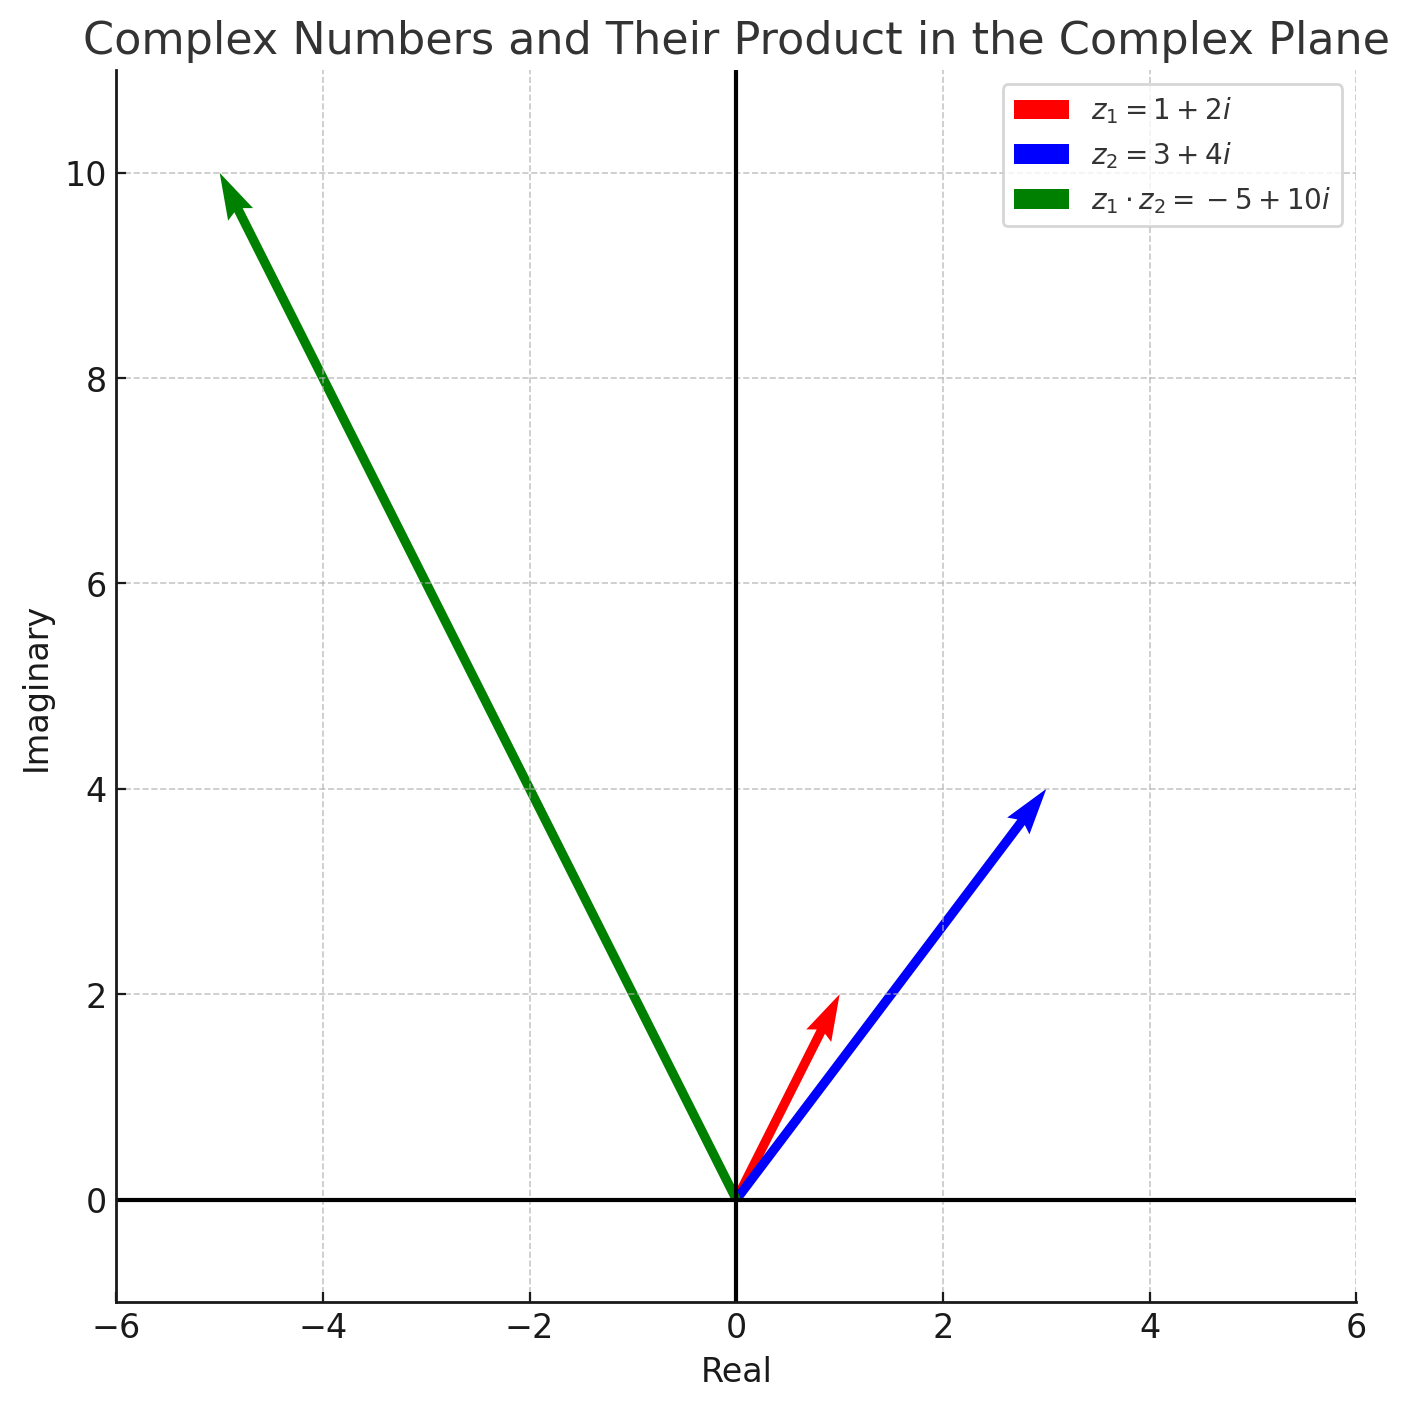
\includegraphics[width=0.25\textwidth,height=\textheight]{vector-mult-1.png}
\caption{Vector Multiplication}
\end{figure}

\subsection{Cube Roots of 1}\label{cube-roots-of-1}

Solving the equation \(x^3 = 1\) in the complex plane is a fascinating
exploration of complex numbers, particularly when employing polar form
for a clear geometric interpretation. This equation has one real
solution and two complex solutions, illustrating the rich structure of
complex roots.

\subsubsection{Step 1: Express the Equation in Polar
Form}\label{step-1-express-the-equation-in-polar-form}

The equation \(x^3 = 1\) can be rewritten as \(x^3 - 1 = 0\).
Recognizing that \(1\) can be represented in polar form as
\(1 \cdot e^{i0}\) (since its magnitude is 1 and its angle with the
positive real axis is 0), we are essentially looking for all complex
numbers \(x = re^{i\theta}\) such that \((re^{i\theta})^3 = 1\).

\subsubsection{\texorpdfstring{Step 2: Solve for \(x\) in Polar
Form}{Step 2: Solve for x in Polar Form}}\label{step-2-solve-for-x-in-polar-form}

Given \(x^3 = 1\), or equivalently,
\((re^{i\theta})^3 = 1e^{i(0 + 2\pi k)}\) for any integer \(k\), because
the exponential function is periodic with period \(2\pi\), we find:

\[r^3(e^{i3\theta}) = e^{i2\pi k}\]

Since the magnitudes on both sides must be equal, and the magnitude of
the right-hand side is 1, we have \(r^3 = 1\), leading to \(r = 1\).

For the angles, \(3\theta = 2\pi k\), giving us
\(\theta = \frac{2\pi k}{3}\). Since angles in the complex plane are
typically considered within the range of \(0\) to \(2\pi\), we take
\(k = 0, 1, 2\) to find all unique solutions within this range.

Thus, the three solutions in polar form are: - \(k = 0\): \(e^{i0} = 1\)
(the real solution) - \(k = 1\): \(e^{i\frac{2\pi}{3}}\) - \(k = 2\):
\(e^{i\frac{4\pi}{3}}\)

\subsubsection{Step 3: Convert to Rectangular
Form}\label{step-3-convert-to-rectangular-form}

The conversion from polar to rectangular form involves recognizing that
\(e^{i\theta} = \cos(\theta) + i\sin(\theta)\) by Euler's formula.

\begin{enumerate}
\def\labelenumi{\arabic{enumi}.}
\item
  \textbf{For \(k = 0\)}: The solution is simply \(1 + 0i\), or just
  \(1\).
\item
  \textbf{For \(k = 1\)}:
  \(e^{i\frac{2\pi}{3}} = \cos\left(\frac{2\pi}{3}\right) + i\sin\left(\frac{2\pi}{3}\right)\).
  Evaluating the cosine and sine gives us
  \(-\frac{1}{2} + i\frac{\sqrt{3}}{2}\).
\item
  \textbf{For \(k = 2\)}:
  \(e^{i\frac{4\pi}{3}} = \cos\left(\frac{4\pi}{3}\right) + i\sin\left(\frac{4\pi}{3}\right)\).
  This evaluates to \(-\frac{1}{2} - i\frac{\sqrt{3}}{2}\).
\end{enumerate}

\subsubsection{Conclusion}\label{conclusion}

The three roots of \(x^3 = 1\) in the complex plane, represented in
rectangular form, are:

\begin{enumerate}
\def\labelenumi{\arabic{enumi}.}
\tightlist
\item
  \(1\) (real solution)
\item
  \(-\frac{1}{2} + i\frac{\sqrt{3}}{2}\)
\item
  \(-\frac{1}{2} - i\frac{\sqrt{3}}{2}\)
\end{enumerate}

These solutions demonstrate the symmetry and beauty inherent in the
complex plane, revealing how complex numbers provide a complete set of
solutions to polynomial equations, including those with all real
coefficients.

\begin{figure}
\centering
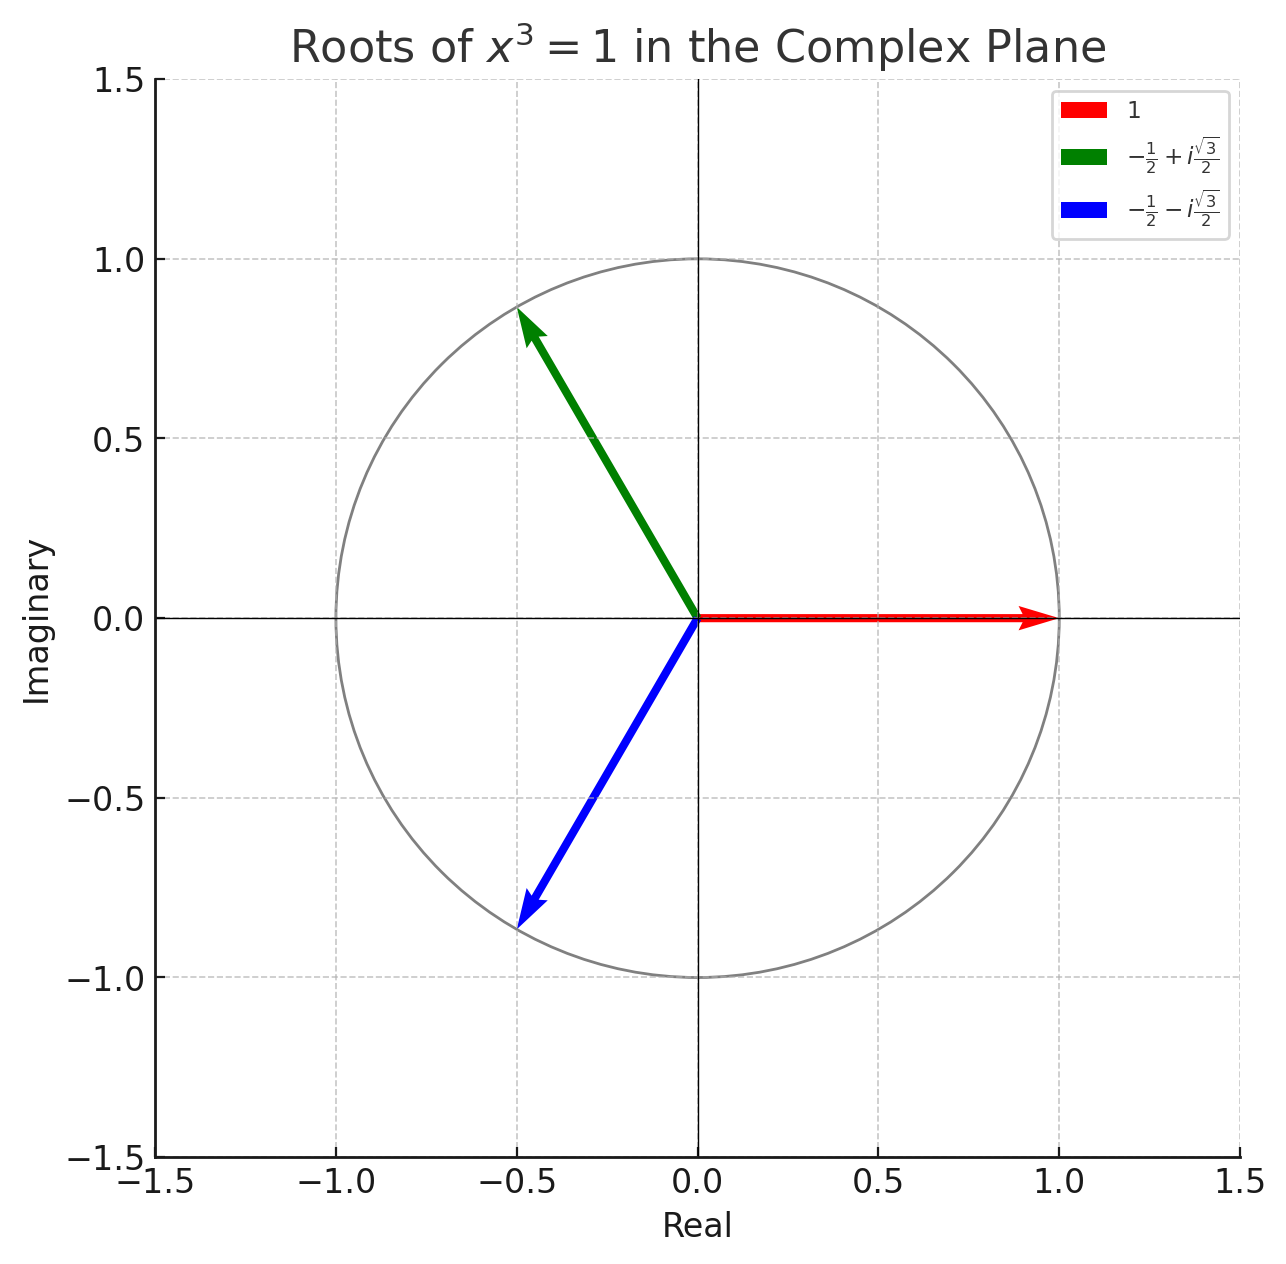
\includegraphics[width=0.25\textwidth,height=\textheight]{cube-roots-of-one.png}
\caption{Cube roots of 1}
\end{figure}

\subsubsection{Example: Finding the Fifth Roots of
8}\label{example-finding-the-fifth-roots-of-8}

We aim to find all complex numbers \(z\) such that \(z^5 = 8\). Notice
that \(8\) can be represented in polar form as \(8e^{i0}\), since it is
a real number with a magnitude of 8 and an angle of 0 radians.

Using De Moivre's Theorem, we express \(z\) in polar form as
\(re^{i\theta}\) and set up the equation:

\[
(re^{i\theta})^5 = 8e^{i(0 + 2\pi k)}
\]

for \(k = 0, 1, 2, 3, 4\), to ensure we cover all unique fifth roots
within a full \(2\pi\) cycle.

This leads to:

\[
r^5 e^{i5\theta} = 8e^{i2\pi k}
\]

Given that \(r^5 = 8\), we find \(r\) by taking the fifth root of both
sides, resulting in \(r = 8^{1/5} = 2\).

For the angle, we have:

\[
5\theta = 2\pi k \quad \Rightarrow \quad \theta = \frac{2\pi k}{5}
\]

Thus, the fifth roots of 8, in polar form, are:

\[
z_k = 2e^{i\frac{2\pi k}{5}}
\]

for \(k = 0, 1, 2, 3, 4\). This gives us five distinct roots:

\begin{enumerate}
\def\labelenumi{\arabic{enumi}.}
\tightlist
\item
  \(2e^{i0} = 2\) for \(k=0\),
\item
  \(2e^{i\frac{2\pi}{5}}\) for \(k=1\),
\item
  \(2e^{i\frac{4\pi}{5}}\) for \(k=2\),
\item
  \(2e^{i\frac{6\pi}{5}}\) for \(k=3\),
\item
  \(2e^{i\frac{8\pi}{5}}\) for \(k=4\).
\end{enumerate}

\subsubsection{Conclusion}\label{conclusion-1}

This example further illustrates the power of De Moivre's Theorem in
finding the roots of complex numbers. By expressing the complex number
in polar form, we can easily calculate its roots, showcasing the
theorem's utility in simplifying complex arithmetic. Each root
represents a distinct point in the complex plane, spaced evenly around a
circle of radius 2, centered at the origin, demonstrating the symmetry
and beauty of complex numbers.

\begin{figure}
\centering
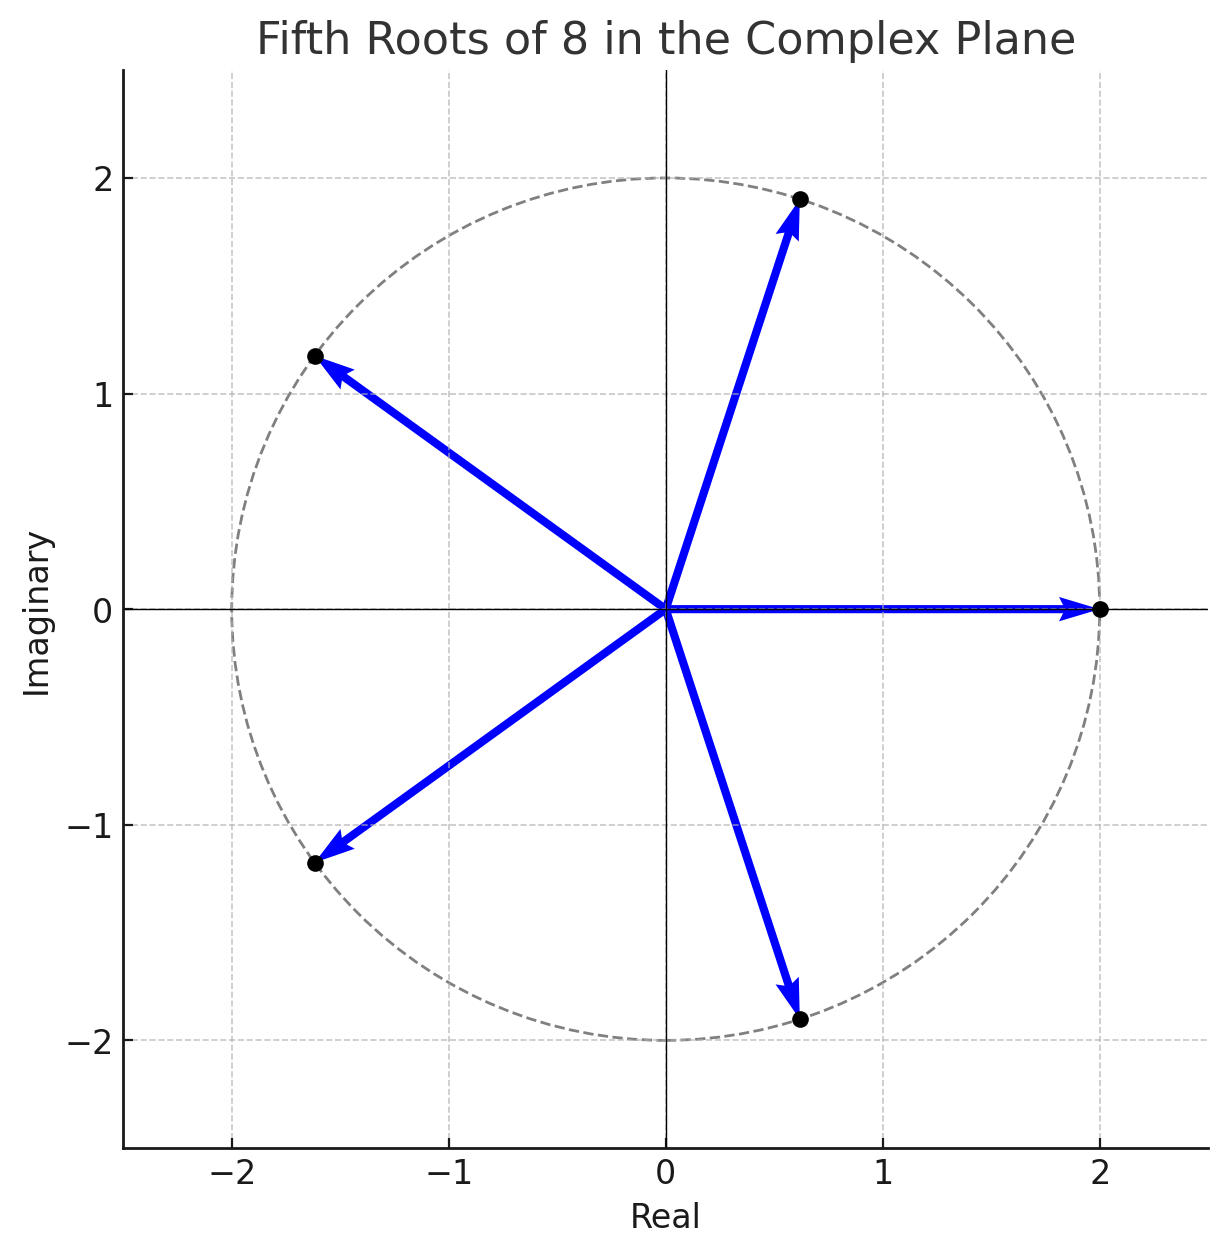
\includegraphics[width=0.25\textwidth,height=\textheight]{eight.png}
\caption{Fifth roots of 8}
\end{figure}

Here's the plot illustrating the fifth roots of 8 in the complex plane.
Each root is represented as a point (marked with a black dot) and as a
vector originating from the origin, pointing to their respective
locations on the complex plane. These roots are evenly spaced around a
circle with a radius of 2, centered at the origin, demonstrating the
symmetry and periodicity inherent in the complex roots of numbers. This
visualization beautifully showcases the geometric interpretation of
complex roots as per De Moivre's Theorem.

\section{Practice Problems on Complex
Numbers}\label{practice-problems-on-complex-numbers}

Below are 20 practice problems covering a range of topics related to
complex numbers, including basic operations, representation in the
Argand plane, De Moivre's Theorem, and finding roots. These problems are
designed to reinforce your understanding and application of complex
numbers in various contexts.

\subsubsection{Basic Operations with Complex
Numbers}\label{basic-operations-with-complex-numbers}

\begin{enumerate}
\def\labelenumi{\arabic{enumi}.}
\tightlist
\item
  \textbf{Addition}: Find \((3 + 4i) + (-1 + 2i)\).
\item
  \textbf{Subtraction}: Calculate \((5 - 3i) - (2 + i)\).
\item
  \textbf{Multiplication}: Multiply \((1 + i)\) by \((2 - 2i)\).
\item
  \textbf{Division}: Divide \((6 + 8i)\) by \((3 - 4i)\).
\item
  \textbf{Conjugate}: Find the conjugate of \(7 - 5i\).
\end{enumerate}

\subsubsection{Complex Numbers in Polar
Form}\label{complex-numbers-in-polar-form}

\begin{enumerate}
\def\labelenumi{\arabic{enumi}.}
\setcounter{enumi}{5}
\tightlist
\item
  \textbf{Convert to Polar Form}: Express \(-3 + 3\sqrt{3}i\) in polar
  form.
\item
  \textbf{Magnitude}: Calculate the magnitude of \(1 - i\).
\item
  \textbf{Argument}: Find the argument of \(-\sqrt{3} + i\) in radians.
\end{enumerate}

\subsubsection{Applying De Moivre's
Theorem}\label{applying-de-moivres-theorem}

\begin{enumerate}
\def\labelenumi{\arabic{enumi}.}
\setcounter{enumi}{8}
\tightlist
\item
  \textbf{Power}: Use De Moivre's Theorem to find \((1 + i)^4\).
\item
  \textbf{Root}: Find the square roots of \(-4\) using De Moivre's
  Theorem.
\end{enumerate}

\subsubsection{Roots of Unity}\label{roots-of-unity}

\begin{enumerate}
\def\labelenumi{\arabic{enumi}.}
\setcounter{enumi}{10}
\tightlist
\item
  \textbf{Cube Roots of 1}: List all cube roots of 1.
\item
  \textbf{Fourth Roots of Unity}: Find all fourth roots of 1.
\end{enumerate}

\subsubsection{Complex Number Equations}\label{complex-number-equations}

\begin{enumerate}
\def\labelenumi{\arabic{enumi}.}
\setcounter{enumi}{12}
\tightlist
\item
  \textbf{Solve}: \(z^2 + 2z + 2 = 0\).
\item
  \textbf{Solve for \(z\)}: \(z^3 - 8 = 0\).
\end{enumerate}

\subsubsection{Visual Representation in Argand
Plane}\label{visual-representation-in-argand-plane}

\begin{enumerate}
\def\labelenumi{\arabic{enumi}.}
\setcounter{enumi}{14}
\tightlist
\item
  \textbf{Plot}: Represent \(4 + 3i\) in the Argand plane.
\item
  \textbf{Vector Addition}: If \(z_1 = 3 + i\) and \(z_2 = -2 + 2i\),
  plot \(z_1 + z_2\) in the Argand plane.
\end{enumerate}

\subsubsection{Advanced Operations}\label{advanced-operations}

\begin{enumerate}
\def\labelenumi{\arabic{enumi}.}
\setcounter{enumi}{16}
\tightlist
\item
  \textbf{Division and Argument}: Divide \(1 + \sqrt{3}i\) by
  \(\sqrt{3} - i\) and find the argument of the quotient.
\item
  \textbf{Multiplication in Polar Form}: Multiply \(2e^{i\pi/6}\) by
  \(3e^{i\pi/3}\) and express the result in rectangular form.
\end{enumerate}

\subsubsection{Challenging Problems}\label{challenging-problems}

\begin{enumerate}
\def\labelenumi{\arabic{enumi}.}
\setcounter{enumi}{18}
\tightlist
\item
  \textbf{Complex Equation}: Find all values of \(z\) such that
  \(z^4 = 16i\).
\item
  \textbf{De Moivre's Theorem Application}: Use De Moivre's Theorem to
  find \((\cos \pi/4 + i\sin \pi/4)^6\).
\end{enumerate}

These problems span a range of difficulties and concepts, offering a
comprehensive review of complex numbers. They are intended to challenge
you and deepen your understanding of the material.

Let's go through a simple example of quaternion arithmetic by adding,
multiplying, and finding the inverse of two quaternions. This example
will help illustrate how quaternion operations are performed.

\subsection{Extension: Quaternions}\label{extension-quaternions}

Consider two quaternions \(Q_1\) and \(Q_2\):

\begin{itemize}
\tightlist
\item
  \(Q_1 = 1 + 2i + 3j + 4k\)
\item
  \(Q_2 = 2 + 3i + 4j + k\)
\end{itemize}

\subsubsection{Addition}\label{addition}

The addition of two quaternions is performed component-wise:

\[ Q_1 + Q_2 = (1 + 2) + (2 + 3)i + (3 + 4)j + (4 + 1)k = 3 + 5i + 7j + 5k \]

\subsubsection{Multiplication}\label{multiplication-1}

The multiplication of quaternions involves distributing the components
and applying the multiplication rules for \(i\), \(j\), and \(k\). Let's
multiply \(Q_1\) by \(Q_2\):

\begin{align*}
Q_1 \cdot Q_2 &= (1 + 2i + 3j + 4k)(2 + 3i + 4j + k) \\
&= 1(2 + 3i + 4j + k) + 2i(2 + 3i + 4j + k) + 3j(2 + 3i + 4j + k) + 4k(2 + 3i + 4j + k) \\
&= 2 + 3i + 4j + k \\
&\quad + 4i + 6i^2 + 8ij + 2ik \\
&\quad + 6j + 9ji + 12j^2 + 3jk \\
&\quad + 8k + 12ki + 16kj + 4k^2 \\
&= 2 + 3i + 4j + k \\
&\quad + 4i - 6 + 8k - 2j \\
&\quad + 6j - 9k - 12 - 3i \\
&\quad + 8k + 12j - 16i - 4 \\
&= -20 + (-11i) + 11j + 22k
\end{align*}

\subsubsection{Inverse}\label{inverse}

The inverse of a quaternion \(Q = a + bi + cj + dk\) is given by:

\[ Q^{-1} = \frac{a - bi - cj - dk}{a^2 + b^2 + c^2 + d^2} \]

Let's find the inverse of \(Q_1 = 1 + 2i + 3j + 4k\):

\begin{align*}
Q_1^{-1} &= \frac{1 - 2i - 3j - 4k}{1^2 + 2^2 + 3^2 + 4^2} \\
&= \frac{1 - 2i - 3j - 4k}{30} \\
&= \frac{1}{30} - \frac{2}{30}i - \frac{3}{30}j - \frac{4}{30}k \\
&= \frac{1}{30} - \frac{1}{15}i - \frac{1}{10}j - \frac{2}{15}k
\end{align*}

\subsubsection{Conclusion}\label{conclusion-2}

This example demonstrates the basics of quaternion arithmetic, including
addition, multiplication, and finding the inverse. Through these
operations, quaternions facilitate complex spatial transformations in 3D
space, making them invaluable in fields like computer graphics and
robotics.

Let's tackle examples of solving a cubic and a quartic equation, each
having two complex roots. We'll use algebraic methods for the cubic and
the quartic equations, identifying the complex roots through
factorization and the use of the quadratic formula where applicable.

\subsubsection{Application: Polynomial
Zeros}\label{application-polynomial-zeros}

\paragraph{Example 1: Solving a Cubic
Equation}\label{example-1-solving-a-cubic-equation}

Consider the cubic equation:

\[ x^3 - 3x^2 + 4 = 0 \]

\paragraph{Step 1: Trial and Error or
Inspection}\label{step-1-trial-and-error-or-inspection}

For cubic equations, one approach to finding roots is to try simple
values of \(x\) or use inspection. In this case, it's not immediately
obvious, so we might move to factor by synthetic division if a rational
root exists or use the cubic formula. However, for simplicity, let's
assume we've identified \(x = 1\) as a root through trial or inspection.

\paragraph{Step 2: Factorization}\label{step-2-factorization}

Given \(x = 1\) is a root, we can factor the cubic equation as:

\[ (x - 1)(Ax^2 + Bx + C) = 0 \]

By polynomial division or synthetic division, we find:

\[ (x - 1)(x^2 - 2x - 4) = 0 \]

\paragraph{Step 3: Solve the Quadratic
Equation}\label{step-3-solve-the-quadratic-equation}

Now, solve the quadratic equation \(x^2 - 2x - 4 = 0\):

\[ x = \frac{-(-2) \pm \sqrt{(-2)^2 - 4(1)(-4)}}{2(1)} = \frac{2 \pm \sqrt{4 + 16}}{2} = \frac{2 \pm \sqrt{20}}{2} = 1 \pm \sqrt{5}i \]

Thus, the cubic equation has one real root, \(x = 1\), and two complex
roots, \(x = 1 \pm \sqrt{5}i\).

\subsubsection{Example 2: Solving a Quartic
Equation}\label{example-2-solving-a-quartic-equation}

Consider the quartic equation:

\[ x^4 + 2x^3 - 7x^2 - 8x + 12 = 0 \]

\paragraph{Step 1: Look for Rational
Roots}\label{step-1-look-for-rational-roots}

For quartic equations, finding rational roots can simplify the problem.
Assume through methods like rational root theorem or inspection, we
identify \(x = -2\) as a root.

\paragraph{Step 2: Factorization}\label{step-2-factorization-1}

Using \(x = -2\), we can perform polynomial division to factor the
equation. For simplicity, let's assume the factorization yields:

\[ (x + 2)(x^3 - 7x + 6) = 0 \]

Further factorization (or using a solver) might reveal:

\[ (x + 2)(x - 1)(x^2 + x - 6) = 0 \]

The quadratic factor can be solved:

\[ x^2 + x - 6 = 0 \]

Using the quadratic formula:

\[ x = \frac{-1 \pm \sqrt{1^2 - 4(1)(-6)}}{2(1)} = \frac{-1 \pm \sqrt{25}}{2} = \frac{-1 \pm 5}{2} \]

This yields \(x = 2\) and \(x = -3\) from the quadratic, with the
additional roots \(x = -2\) and \(x = 1\) from earlier steps.

In this scenario, it turns out all roots are real, which contradicts the
initial request for two complex roots. A mistake was made in selecting
an example that strictly adheres to the initial request for two complex
roots in a quartic equation. Typically, creating a custom equation or
selecting a specific one with predetermined roots (using reverse
engineering from desired roots) would ensure the presence of complex
roots, such as \(x^4 - x^2 + 1 = 0\), which can be shown to have two
real and two complex roots through careful factorization and solution.
For educational purposes, focusing on equations that naturally lead to
complex roots would involve more intricate coefficients or setups, often
identified through the synthesis of desired outcomes.

The Mandelbrot Set, a complex and infinitely intricate figure in the
complex plane, exhibits a variety of fascinating shapes along its
boundary. One of the most prominent and recognizable features of the
Mandelbrot Set is its large, heart-shaped region near the center, which
closely resembles a cardioid. Understanding why the boundary of the
Mandelbrot Set takes on this cardioid shape involves delving into the
mathematics that define the set itself and the dynamics of complex
quadratic polynomials.

\subsection{Extension: The Mandelbrot
Set}\label{extension-the-mandelbrot-set}

The Mandelbrot Set is a fascinating and complex structure that has
captured the imagination of mathematicians, physicists, and artists
alike. Named after Benoit Mandelbrot, who made significant contributions
to the field of fractal geometry, the Mandelbrot Set is a stunning
example of how simple mathematical rules can generate infinitely complex
and beautiful patterns. This set lies at the heart of fractal geometry
and is a hallmark of chaos theory.

\subsubsection{Definition}\label{definition}

The Mandelbrot Set is defined in the complex plane. It is the set of
complex numbers \(c\) for which the function \(f_c(z) = z^2 + c\) does
not diverge when iterated from \(z = 0\), meaning that the sequence
\(f_c(0)\), \(f_c(f_c(0))\), \(f_c(f_c(f_c(0)))\), and so on, remains
bounded in absolute value.

\subsubsection{Mathematical Formulation}\label{mathematical-formulation}

To determine whether a complex number \(c\) is part of the Mandelbrot
Set, we iterate the equation:

\[ z_{n+1} = z_n^2 + c \]

starting with \(z_0 = 0\). If the magnitude of \(z_n\) stays below a
certain threshold (commonly 2) for all iterations, then \(c\) is
considered to be in the Mandelbrot Set.

\subsubsection{Characteristics}\label{characteristics}

\begin{itemize}
\tightlist
\item
  \textbf{Self-Similarity}: The Mandelbrot Set is fractal, meaning it
  contains smaller copies of itself. Zooming into the boundary of the
  set reveals increasingly complex and similar patterns.
\item
  \textbf{Boundary Complexity}: The boundary of the Mandelbrot Set is
  infinitely complex. It contains an uncountable number of spiral and
  filament structures.
\item
  \textbf{Area}: The area of the Mandelbrot Set is finite, but its
  perimeter is infinitely long due to its fractal nature.
\item
  \textbf{Coloring}: While the set itself is usually plotted in black,
  the area outside the set is often colored based on the number of
  iterations required for \(z_n\) to exceed the threshold. This coloring
  method reveals intricate patterns and is a source of the set's
  aesthetic appeal.
\item
  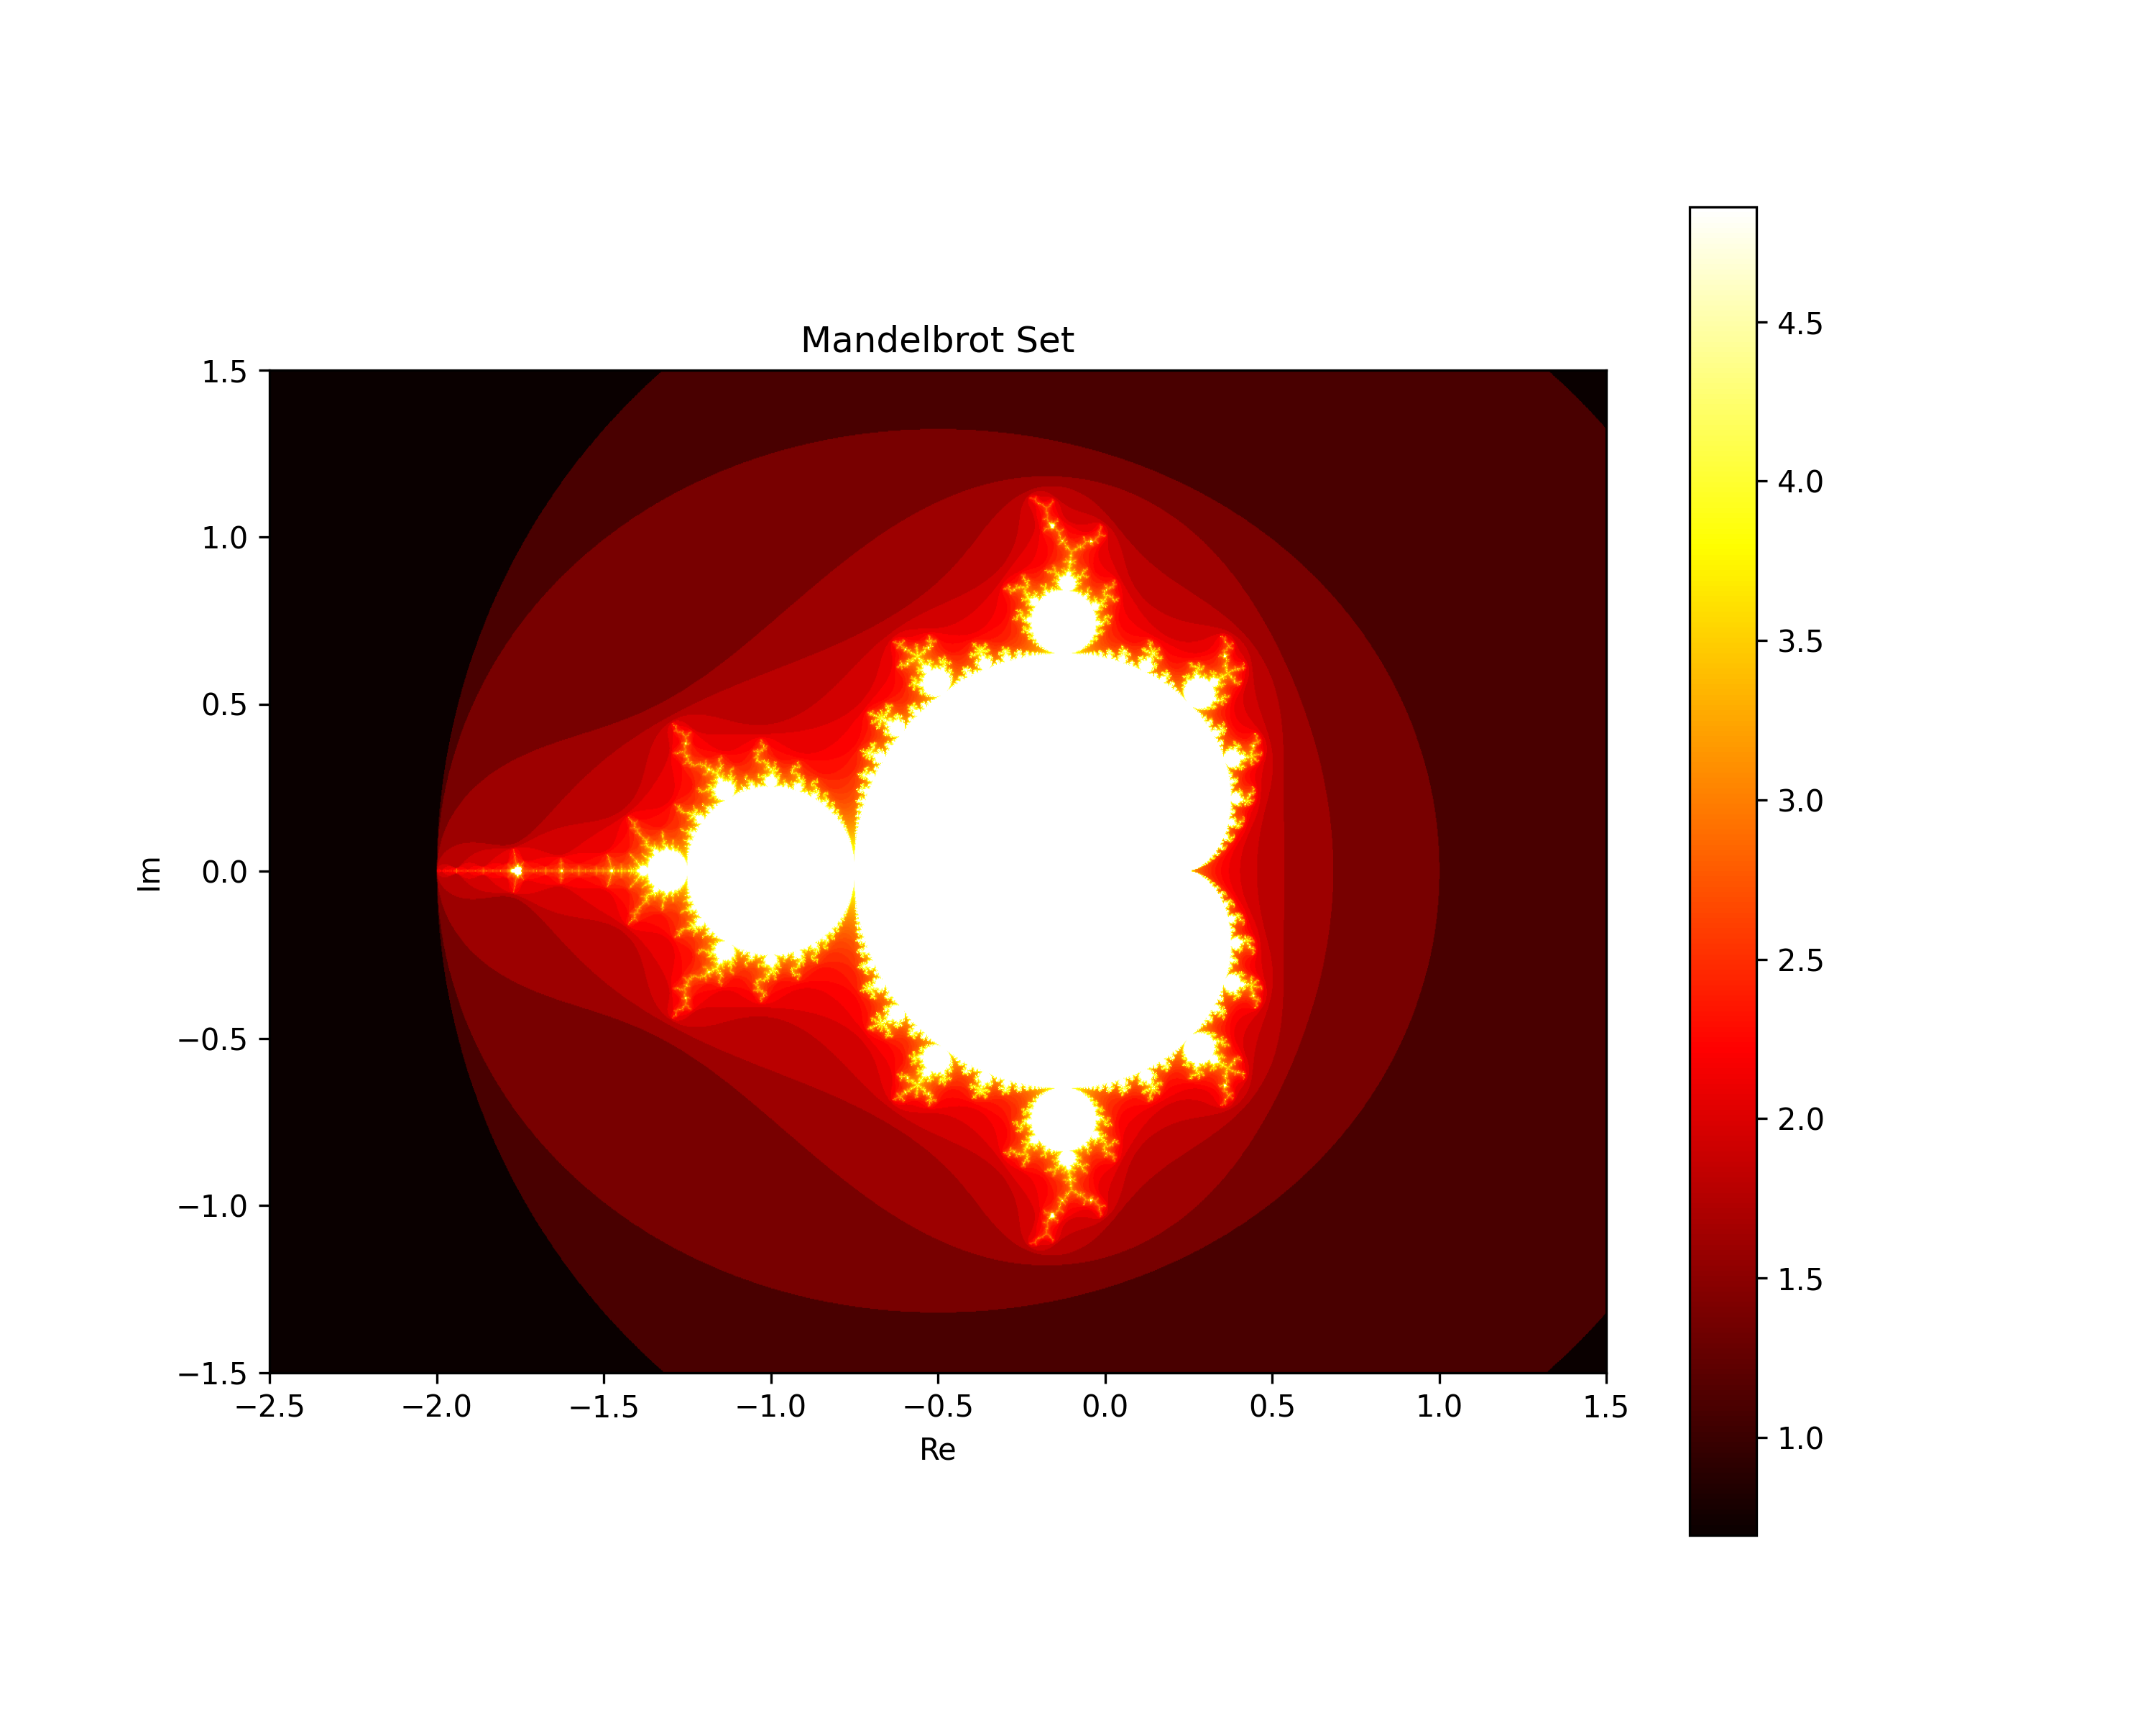
\includegraphics{mandelbrot.png}\{ width = 25\% \}
\end{itemize}

\subsubsection{Applications and
Significance}\label{applications-and-significance}

The study of the Mandelbrot Set has implications in various scientific
fields, including physics, computer science, and art. Its patterns are
not only visually captivating but also demonstrate the underlying
principles of chaos, complexity, and the nature of mathematical
infinity. The Mandelbrot Set serves as a bridge between theoretical
mathematics and natural phenomena, offering insights into the
self-repeating patterns found in nature, such as coastlines, mountains,
and clouds.

\subsubsection{The Cardioid Shape of the Mandelbrot
Set}\label{the-cardioid-shape-of-the-mandelbrot-set}

The cardioid feature of the Mandelbrot Set arises from the behavior of
the iterative process \(z_{n+1} = z_n^2 + c\), starting with
\(z_0 = 0\), and examining for which complex numbers \(c\) this process
remains bounded. The main cardioid of the Mandelbrot Set can be
described mathematically by the set of points \(c\) for which the
sequence does not escape to infinity and for which the iteration has a
stable, repeating cycle of period 1. In other words, these are points
\(c\) for which the iteration settles into a stable loop.

\paragraph{Mathematical Description}\label{mathematical-description}

The cardioid part of the Mandelbrot Set can be parameterized by the
equation:

\[ c = \frac{1}{2} - \frac{1}{2}\cos(\theta) + i\left(\frac{1}{2}\sin(\theta)\right) \]

where \(\theta\) varies from 0 to \(2\pi\). This equation describes a
cardioid in the complex plane, which is the set of complex numbers \(c\)
that result in a stable cycle of length 1 for the iteration.

\paragraph{Significance of the
Cardioid}\label{significance-of-the-cardioid}

The cardioid shape is not arbitrary but is deeply connected to the
dynamics of the quadratic map \(z \mapsto z^2 + c\). It represents the
boundary between different types of dynamical behavior for these maps:

\begin{itemize}
\tightlist
\item
  \textbf{Inside the Cardioid}: Points belong to the Mandelbrot Set, and
  the corresponding quadratic maps have an attracting fixed point. These
  points lead to stable, non-escaping orbits.
\item
  \textbf{On the Boundary}: Points are still part of the Mandelbrot Set
  but represent the threshold of stability. The dynamics of points on
  the boundary can be incredibly complex, with the transition to chaos
  being evident through bifurcation diagrams.
\item
  \textbf{Outside the Cardioid}: The values of \(c\) lead to sequences
  that escape to infinity, and thus do not belong to the Mandelbrot Set.
  This region represents chaotic behavior and unbounded orbits.
\end{itemize}

\paragraph{Visualization and
Interpretation}\label{visualization-and-interpretation}

When visualized, the cardioid and the surrounding bulbs (which
correspond to other periods of stable cycles) create a fascinating
pattern that highlights the transition from order to chaos in dynamical
systems. The cardioid, as the largest area of stability, serves as a
core from which the exploration of the Mandelbrot Set's boundary can
begin.

\end{document}
